\documentclass[12pt,a4paper]{article}

\usepackage[utf8]{inputenc}
\usepackage[T1]{fontenc}
\usepackage[spanish]{babel}
\usepackage[a4paper,margin=2.5cm]{geometry}
\usepackage{enumitem}
\usepackage{graphicx}
\usepackage{hyperref}

\title{Trabajo Práctico Grupal -- Primera Entrega\\Sistema Nacional de Registro de Accidentes Viales}
\author{Franco Odiz, Juan Pablo Saldungaray y Uriel Slavkin}
\date{17/05/2026}

\begin{document}

\maketitle

\section{Introducción}

El presente trabajo desarrolla el diseño de una base de datos para un Registro Único de Accidentes de Tránsito (RUAT). El objetivo es modelar la información necesaria para registrar siniestros viales, personas involucradas, vehículos, antecedentes, peritajes y características del entorno, de modo de permitir tanto el almacenamiento operativo como la posterior explotación analítica de los datos.

La propuesta se apoya en un modelado conceptual del dominio y en su posterior transformación al modelo relacional, con especial atención a la eliminación de redundancia, la explicitación de restricciones y la posibilidad de realizar consultas de interés para la toma de decisiones.

El dominio elegido ---el registro de accidentes viales--- resultó especialmente rico para trabajar los conceptos de la materia. A diferencia de dominios más lineales, este requirió modelar un mismo hecho (el siniestro) relacionado con múltiples entidades independientes (personas, vehículos, tramos viales) a través de vínculos que en algunos casos son ternarios. Eso nos obligó a tomar decisiones de diseño no triviales que se desarrollan a lo largo de este informe.

\section{Análisis del dominio y requerimientos}

El primer paso fue identificar qué información necesita registrar el sistema y con qué nivel de detalle. Partimos del enunciado provisto por la cátedra y lo complementamos con decisiones propias para cubrir casos que el enunciado dejaba abiertos.

\subsection*{Requerimientos funcionales identificados}

\begin{itemize}[leftmargin=*]
    \item Registrar cada siniestro con su fecha, hora, lugar, denuncia policial, tipo de accidente y tipo de colisión.
    \item Asociar cada siniestro a un tramo o lugar vial relevante para poder analizar accidentes por tipo de camino.
    \item Registrar personas involucradas en los hechos, incluyendo conductores, acompañantes, testigos y víctimas no vehiculares.
    \item Registrar vehículos involucrados, junto con información del parque automotor, categoría, antigüedad, aseguradora y cobertura.
    \item Registrar informes técnicos, estudios y peritajes vinculados con cada siniestro.
    \item Registrar condiciones contextuales del hecho: estado de la vía, pavimento, iluminación, clima y elementos de seguridad peatonal.
    \item Registrar antecedentes asociados a las personas: licencias de conducir, infracciones y antecedentes penales.
    \item Permitir consultas que sirvan para describir y analizar el fenómeno, por ejemplo:
    \begin{itemize}
        \item cantidad de accidentes por tipo de camino;
        \item cantidad de accidentes por tipo de vehículo;
        \item accidentes asociados a ciertas fallas humanas;
        \item presencia de antecedentes o licencias vencidas en personas involucradas.
    \end{itemize}
\end{itemize}

\subsection*{Decisiones de modelado incorporadas}

Además de los requerimientos explícitos, durante el análisis identificamos situaciones que el enunciado no cubría con precisión y que requerían una decisión de diseño.

\begin{itemize}[leftmargin=*]
    \item \textbf{Separar \texttt{PERSONA} y \texttt{VEHICULO} como entidades independientes.} Ambas pueden participar en múltiples siniestros a lo largo del tiempo. Si las datos de una persona o vehículo estuvieran dentro de la tabla de siniestros, deberían repetirse en cada hecho en que intervengan, generando redundancia.

    \item \textbf{Modelar la participación como relación ternaria.} La vinculación entre una persona, un vehículo y un siniestro no puede representarse correctamente con dos relaciones binarias separadas. El rol de una persona (conductor o acompañante) es específico de esa terna concreta: una misma persona puede ser conductora en un siniestro y acompañante en otro, y puede hacerlo en distintos vehículos. Por eso se creó \texttt{PARTICIPACION\_VEHICULAR} como relación ternaria.

    \item \textbf{Separar los informes técnicos del siniestro.} Un mismo hecho puede originar uno o varios estudios emitidos por distintos organismos en distintos momentos. Almacenar las condiciones del hecho directamente en la tabla \texttt{SINIESTRO} haría imposible registrar más de un informe por siniestro sin duplicar datos.

    \item \textbf{Modelar la infraestructura vial mediante una entidad propia.} Contar con una tabla \texttt{TRAMO\_VIAL} separada permite no solo registrar dónde ocurrió cada accidente, sino también analizar estadísticas por tipo de camino o jurisdicción sin depender de texto libre en cada siniestro.
\end{itemize}

\section{Modelo conceptual}

A continuación se describe el modelo conceptual del dominio. Se identifican las entidades con sus atributos y las interrelaciones entre ellas.

\subsection*{Diagrama Entidad--Interrelación}

\begin{figure}[h]
    \centering
    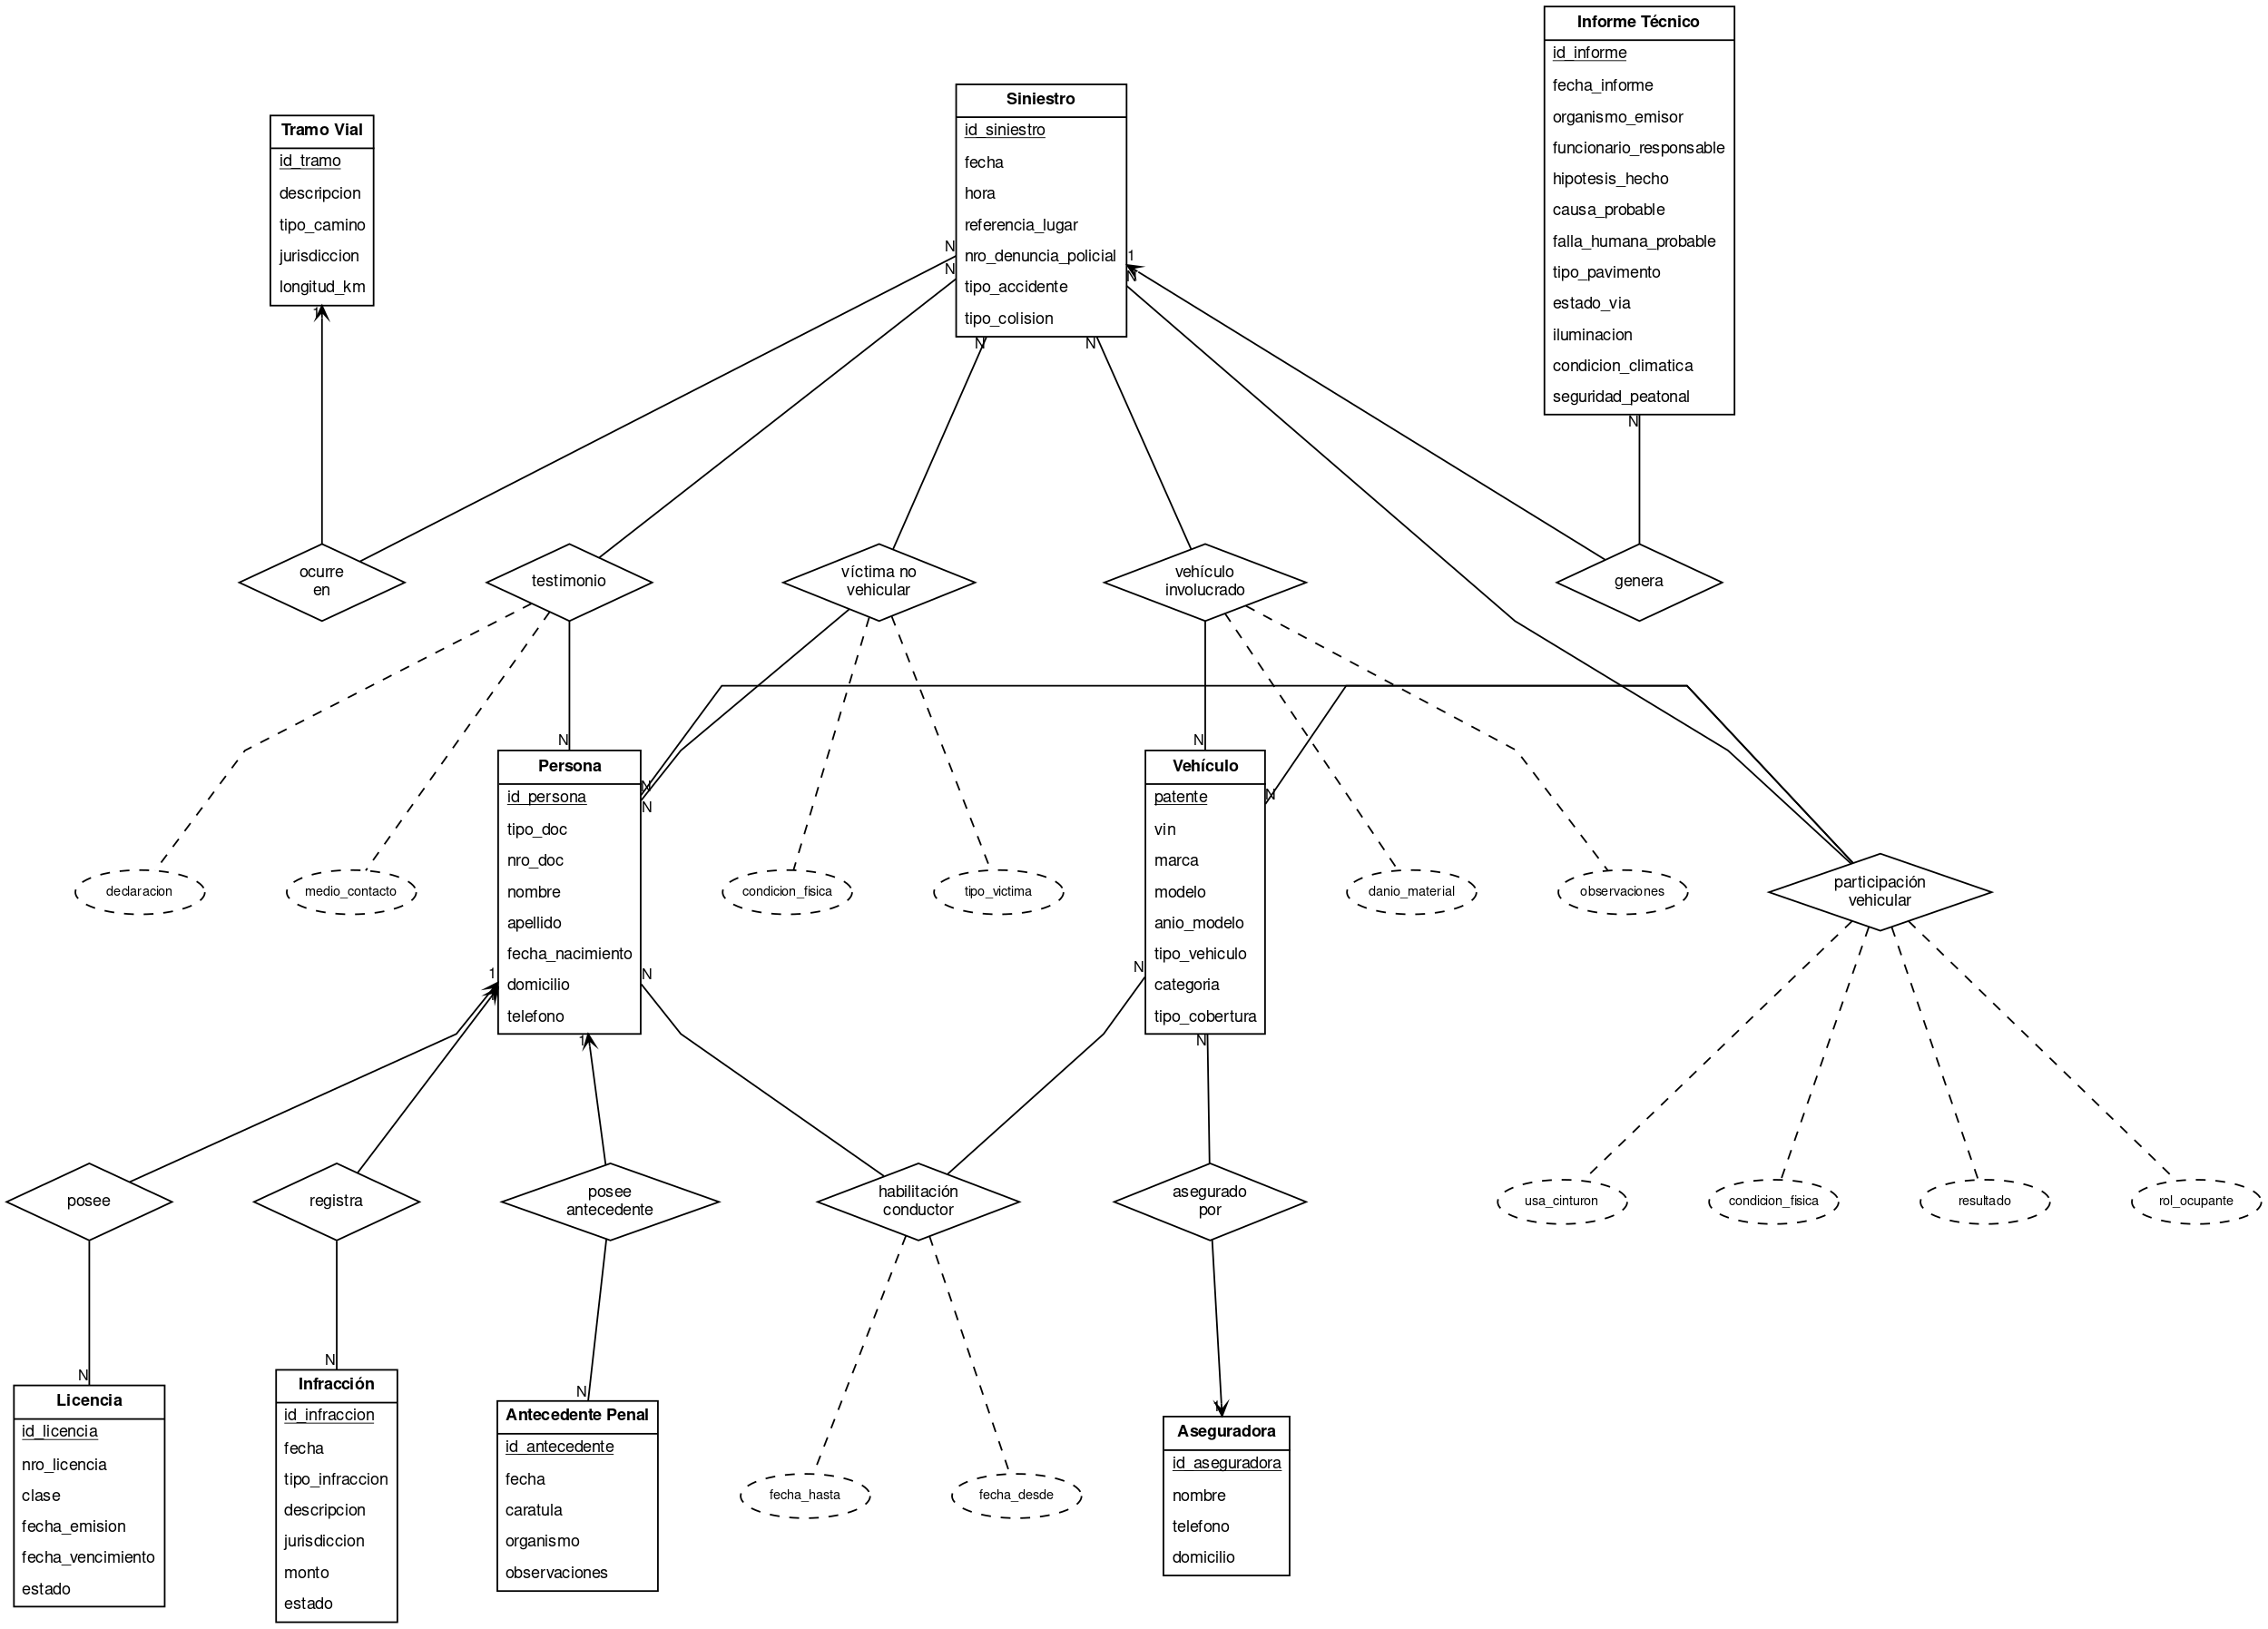
\includegraphics[width=\textwidth]{der_ruat.png}
    \caption{Diagrama Entidad--Interrelación del RUAT (notación Chen)}
\end{figure}

El diagrama muestra las entidades principales (rectángulos azules), las tablas asociativas que surgen de relaciones N:M o ternarias (rectángulos verdes con borde punteado) y las relaciones nominales con su cardinalidad (rombos).

\subsection*{Entidades}

\begin{itemize}[leftmargin=*]
    \item \textbf{SINIESTRO}(\underline{id\_siniestro}, fecha, hora, referencia\_lugar, nro\_denuncia\_policial, tipo\_accidente, tipo\_colision)
    \item \textbf{TRAMO\_VIAL}(\underline{id\_tramo}, descripcion, tipo\_camino, jurisdiccion, longitud\_km)
    \item \textbf{PERSONA}(\underline{id\_persona}, tipo\_doc, nro\_doc, nombre, apellido, fecha\_nacimiento, domicilio, telefono)
    \item \textbf{LICENCIA}(\underline{id\_licencia}, nro\_licencia, clase, fecha\_emision, fecha\_vencimiento, estado)
    \item \textbf{INFRACCION}(\underline{id\_infraccion}, fecha, tipo\_infraccion, descripcion, jurisdiccion, monto, estado)
    \item \textbf{ANTECEDENTE\_PENAL}(\underline{id\_antecedente}, fecha, caratula, organismo, observaciones)
    \item \textbf{VEHICULO}(\underline{patente}, vin, marca, modelo, anio\_modelo, tipo\_vehiculo, categoria, tipo\_cobertura)
    \item \textbf{ASEGURADORA}(\underline{id\_aseguradora}, nombre, telefono, domicilio)
    \item \textbf{INFORME\_TECNICO}(\underline{id\_informe}, fecha\_informe, organismo\_emisor, funcionario\_responsable, hipotesis\_hecho, causa\_probable, falla\_humana\_probable, tipo\_pavimento, estado\_via, iluminacion, condicion\_climatica, seguridad\_peatonal)
\end{itemize}

\subsection*{Relaciones y participación}

Para cada relación se indica la cardinalidad y el tipo de participación de cada entidad. La \textbf{participación total} (representada con línea doble en Chen) implica que toda instancia de esa entidad debe participar en al menos una ocurrencia de la relación. La \textbf{participación parcial} (línea simple) implica que puede haber instancias que no participen.

\begin{itemize}[leftmargin=*]
    \item \textbf{OCURRE\_EN} entre \texttt{SINIESTRO} y \texttt{TRAMO\_VIAL}: cardinalidad N:1. Un tramo vial puede estar asociado a muchos siniestros; cada siniestro se registra en un único tramo vial principal. Cuando el hecho abarca más de un tramo, se registra el de mayor relevancia. \emph{Participación: total desde \texttt{SINIESTRO} (todo siniestro debe tener un tramo asignado), parcial desde \texttt{TRAMO\_VIAL} (un tramo puede no tener siniestros registrados todavía).}

    \item \textbf{GENERA} entre \texttt{SINIESTRO} e \texttt{INFORME\_TECNICO}: cardinalidad 1:N. Un siniestro puede generar cero, uno o varios informes; cada informe corresponde a un único siniestro. La separación permite que distintos organismos periciales emitan sus propios informes sobre el mismo hecho. \emph{Participación: parcial desde \texttt{SINIESTRO} (puede haber siniestros sin informe técnico aún, por ejemplo cuando la investigación está pendiente), total desde \texttt{INFORME\_TECNICO} (todo informe debe estar asociado a algún siniestro concreto).}

    \item \textbf{VEHICULO\_INVOLUCRADO} entre \texttt{SINIESTRO} y \texttt{VEHICULO}: relación N:M. Un siniestro puede involucrar varios vehículos y un mismo vehículo puede haber estado en varios siniestros. La tabla asociativa registra datos propios del vínculo, como el daño material. \emph{Participación: total desde \texttt{SINIESTRO} (todo siniestro debe tener al menos un vehículo involucrado para ser registrado como tal), parcial desde \texttt{VEHICULO} (un vehículo puede existir en el padrón sin haber estado nunca en un siniestro).}

    \item \textbf{PARTICIPACION\_VEHICULAR} entre \texttt{SINIESTRO}, \texttt{PERSONA} y \texttt{VEHICULO}: relación ternaria N:N:N. Representa a una persona asociada a un vehículo dentro de un siniestro determinado, con atributos propios del vínculo (rol, uso de cinturón, condición física, resultado). \emph{Participación: parcial desde las tres entidades. Un siniestro puede tener vehículos sin conductores identificados; una persona puede estar registrada en el sistema sin haber participado en ningún siniestro; un vehículo puede estar involucrado sin que se hayan determinado sus ocupantes.}

    \item \textbf{TESTIMONIO} entre \texttt{SINIESTRO} y \texttt{PERSONA}: relación N:M. Registra declaraciones de personas que no viajaban en ningún vehículo involucrado. \emph{Participación: parcial desde ambas entidades. No todo siniestro cuenta con testigos, y no toda persona ha prestado testimonio en algún hecho.}

    \item \textbf{VICTIMA\_NO\_VEHICULAR} entre \texttt{SINIESTRO} y \texttt{PERSONA}: relación N:M. Modela personas afectadas que no participaban como ocupantes de vehículos, como peatones o ciclistas. \emph{Participación: parcial desde ambas entidades. Los atropellos generan víctimas no vehiculares, pero la mayoría de los siniestros involucran solo vehículos. No toda persona del sistema fue víctima de un siniestro.}

    \item \textbf{POSEE} entre \texttt{PERSONA} y \texttt{LICENCIA}: relación 1:N. Una persona puede tener varias licencias a lo largo del tiempo (por renovaciones o cambios de categoría). \emph{Participación: parcial desde \texttt{PERSONA} (puede haber personas registradas sin licencia en el sistema, por ejemplo víctimas peatonales), total desde \texttt{LICENCIA} (toda licencia debe pertenecer a alguna persona).}

    \item \textbf{REGISTRA} entre \texttt{PERSONA} e \texttt{INFRACCION}: relación 1:N. Una persona puede acumular múltiples infracciones de tránsito. \emph{Participación: parcial desde \texttt{PERSONA} (la mayoría de las personas no tienen infracciones), total desde \texttt{INFRACCION} (toda infracción debe estar asociada a una persona responsable).}

    \item \textbf{POSEE\_ANTECEDENTE} entre \texttt{PERSONA} y \texttt{ANTECEDENTE\_PENAL}: relación 1:N. Los antecedentes penales son de la persona y se mantienen independientemente de los siniestros. \emph{Participación: parcial desde \texttt{PERSONA} (pocos individuos tienen antecedentes penales), total desde \texttt{ANTECEDENTE\_PENAL} (todo antecedente debe pertenecer a una persona).}

    \item \textbf{HABILITACION\_CONDUCCION} entre \texttt{PERSONA} y \texttt{VEHICULO}: relación N:M con atributo temporal (fecha\_desde, fecha\_hasta). Registra si una persona está formalmente habilitada para conducir un vehículo determinado. No implica que esa persona haya conducido el vehículo en ningún siniestro en particular; eso lo modela \texttt{PARTICIPACION\_VEHICULAR}. \emph{Participación: parcial desde ambas entidades. No toda persona del sistema tiene habilitaciones registradas para vehículos específicos, y no todo vehículo tiene habilitaciones asociadas.}

    \item \textbf{ASEGURADO\_POR} entre \texttt{VEHICULO} y \texttt{ASEGURADORA}: relación N:1. Se registra la aseguradora y cobertura vigentes al momento del hecho. \emph{Participación: total desde \texttt{VEHICULO} (todo vehículo registrado en el sistema debe tener una aseguradora asignada, dado que la cobertura es obligatoria), parcial desde \texttt{ASEGURADORA} (una aseguradora puede existir en el sistema sin que haya vehículos asignados todavía).}
\end{itemize}

\subsection*{Decisiones de participación: dos ejemplos}

La distinción entre participación total y parcial tiene consecuencias prácticas en el diseño. Se destacan dos casos representativos.

\textbf{Ejemplo 1 --- OCURRE\_EN (total desde SINIESTRO).} La participación total de \texttt{SINIESTRO} en \texttt{OCURRE\_EN} se traduce directamente en que el atributo \texttt{id\_tramo} en la tabla \texttt{SINIESTRO} es \texttt{NOT NULL}. No tiene sentido registrar un siniestro sin ubicarlo en alguna vía. Si la participación fuera parcial, \texttt{id\_tramo} podría ser nulo y el modelo perdería capacidad de análisis geográfico. Esta decisión de diseño queda reflejada tanto en el diagrama E-R (línea doble) como en el DDL (\texttt{id\_tramo INTEGER NOT NULL REFERENCES tramo\_vial}).

\textbf{Ejemplo 2 --- GENERA (parcial desde SINIESTRO).} La participación parcial de \texttt{SINIESTRO} en \texttt{GENERA} refleja que un siniestro puede existir en el sistema antes de que se haya emitido algún informe técnico. En la práctica, el hecho se registra inmediatamente (con fecha, hora, lugar y vehículos), pero el informe pericial puede demorar días o semanas. Si la participación fuera total, no podríamos insertar un siniestro hasta tener al menos un informe, lo que bloquearía el flujo de trabajo operativo. Esta flexibilidad se implementa simplemente no imponiendo restricciones adicionales: basta con que la clave foránea en \texttt{INFORME\_TECNICO} apunte a \texttt{SINIESTRO}, sin ninguna restricción inversa.

\section{Modelo lógico: esquema relacional}

A partir del modelo conceptual se obtiene el siguiente esquema relacional. Las claves primarias se indican subrayadas en la lista de atributos y también explícitamente con \texttt{PK}. Las claves foráneas se indican con \texttt{FK} y la referencia correspondiente.

El pasaje del modelo E-R al relacional siguió las siguientes reglas: las entidades fuertes generan tablas propias; las relaciones N:M se descomponen en tablas asociativas con clave primaria compuesta por las claves de ambas entidades participantes; las relaciones 1:N se resuelven incorporando la clave de la entidad del lado ``uno'' como clave foránea en la tabla del lado ``N''.

\begin{enumerate}[leftmargin=*]
    \item \texttt{TRAMO\_VIAL(\underline{id\_tramo}, descripcion, tipo\_camino, jurisdiccion, longitud\_km)}\\
    PK: \texttt{id\_tramo}

    \item \texttt{SINIESTRO(\underline{id\_siniestro}, fecha, hora, id\_tramo, referencia\_lugar, nro\_denuncia\_policial, tipo\_accidente, tipo\_colision)}\\
    PK: \texttt{id\_siniestro}\\
    FK: \texttt{id\_tramo} $\rightarrow$ \texttt{TRAMO\_VIAL(id\_tramo)}

    \item \texttt{INFORME\_TECNICO(\underline{id\_informe}, id\_siniestro, fecha\_informe, organismo\_emisor, funcionario\_responsable, hipotesis\_hecho, causa\_probable, falla\_humana\_probable, tipo\_pavimento, estado\_via, iluminacion, condicion\_climatica, seguridad\_peatonal)}\\
    PK: \texttt{id\_informe}\\
    FK: \texttt{id\_siniestro} $\rightarrow$ \texttt{SINIESTRO(id\_siniestro)}

    \item \texttt{PERSONA(\underline{id\_persona}, tipo\_doc, nro\_doc, nombre, apellido, fecha\_nacimiento, domicilio, telefono)}\\
    PK: \texttt{id\_persona}

    \item \texttt{LICENCIA(\underline{id\_licencia}, id\_persona, nro\_licencia, clase, fecha\_emision, fecha\_vencimiento, estado)}\\
    PK: \texttt{id\_licencia}\\
    FK: \texttt{id\_persona} $\rightarrow$ \texttt{PERSONA(id\_persona)}

    \item \texttt{INFRACCION(\underline{id\_infraccion}, id\_persona, fecha, tipo\_infraccion, descripcion, jurisdiccion, monto, estado)}\\
    PK: \texttt{id\_infraccion}\\
    FK: \texttt{id\_persona} $\rightarrow$ \texttt{PERSONA(id\_persona)}

    \item \texttt{ANTECEDENTE\_PENAL(\underline{id\_antecedente}, id\_persona, fecha, caratula, organismo, observaciones)}\\
    PK: \texttt{id\_antecedente}\\
    FK: \texttt{id\_persona} $\rightarrow$ \texttt{PERSONA(id\_persona)}

    \item \texttt{ASEGURADORA(\underline{id\_aseguradora}, nombre, telefono, domicilio)}\\
    PK: \texttt{id\_aseguradora}

    \item \texttt{VEHICULO(\underline{patente}, vin, marca, modelo, anio\_modelo, tipo\_vehiculo, categoria, tipo\_cobertura, id\_aseguradora)}\\
    PK: \texttt{patente}\\
    FK: \texttt{id\_aseguradora} $\rightarrow$ \texttt{ASEGURADORA(id\_aseguradora)}

    \item \texttt{HABILITACION\_CONDUCCION(\underline{id\_persona, patente, fecha\_desde}, fecha\_hasta)}\\
    PK: \texttt{(id\_persona, patente, fecha\_desde)}\\
    FK: \texttt{id\_persona} $\rightarrow$ \texttt{PERSONA(id\_persona)}\\
    FK: \texttt{patente} $\rightarrow$ \texttt{VEHICULO(patente)}

    \item \texttt{VEHICULO\_INVOLUCRADO(\underline{id\_siniestro, patente}, danio\_material, observaciones)}\\
    PK: \texttt{(id\_siniestro, patente)}\\
    FK: \texttt{id\_siniestro} $\rightarrow$ \texttt{SINIESTRO(id\_siniestro)}\\
    FK: \texttt{patente} $\rightarrow$ \texttt{VEHICULO(patente)}

    \item \texttt{PARTICIPACION\_VEHICULAR(\underline{id\_siniestro, id\_persona, patente}, rol\_ocupante, usa\_cinturon, condicion\_fisica, resultado)}\\
    PK: \texttt{(id\_siniestro, id\_persona, patente)}\\
    FK: \texttt{id\_persona} $\rightarrow$ \texttt{PERSONA(id\_persona)}\\
    FK: \texttt{(id\_siniestro, patente)} $\rightarrow$ \texttt{VEHICULO\_INVOLUCRADO(id\_siniestro, patente)}

    \item \texttt{TESTIMONIO(\underline{id\_siniestro, id\_persona}, declaracion, medio\_contacto)}\\
    PK: \texttt{(id\_siniestro, id\_persona)}\\
    FK: \texttt{id\_siniestro} $\rightarrow$ \texttt{SINIESTRO(id\_siniestro)}\\
    FK: \texttt{id\_persona} $\rightarrow$ \texttt{PERSONA(id\_persona)}

    \item \texttt{VICTIMA\_NO\_VEHICULAR(\underline{id\_siniestro, id\_persona}, tipo\_victima, condicion\_fisica, observaciones)}\\
    PK: \texttt{(id\_siniestro, id\_persona)}\\
    FK: \texttt{id\_siniestro} $\rightarrow$ \texttt{SINIESTRO(id\_siniestro)}\\
    FK: \texttt{id\_persona} $\rightarrow$ \texttt{PERSONA(id\_persona)}
\end{enumerate}

\section{Sustento lógico y normalización}

El diseño busca reducir redundancias y anomalías de actualización, inserción y eliminación. A continuación se justifica el cumplimiento de BCNF para las tablas más representativas.

\subsection*{Principios generales aplicados}

\begin{itemize}[leftmargin=*]
    \item Los datos del siniestro se almacenan una sola vez en \texttt{SINIESTRO}. Las condiciones contextuales del hecho (estado de la vía, clima, iluminación) quedan en \texttt{INFORME\_TECNICO} porque son certificadas por el organismo que emite el peritaje, no por el sistema de registro en el momento del hecho.
    \item Los datos permanentes de personas y vehículos se separan de sus participaciones en hechos concretos. Esto evita repetir datos como nombre, apellido o marca del vehículo cada vez que una entidad interviene en un siniestro.
    \item Los antecedentes de las personas (licencias, infracciones, penales) se modelan en tablas específicas. Pertenecen a la persona con independencia de los siniestros en que haya participado.
    \item Las relaciones N:M se descomponen en tablas asociativas para evitar atributos multivaluados.
    \item La participación persona--vehículo--siniestro se modela explícitamente como relación ternaria porque no puede representarse correctamente con una sola relación binaria.
\end{itemize}

\subsection*{Verificación de BCNF}

Una relación está en BCNF si, para toda dependencia funcional no trivial $X \rightarrow Y$, el determinante $X$ es superclave. A continuación se justifica esto para las tablas con clave compuesta, que son las más susceptibles de violar BCNF.

\textbf{VEHICULO\_INVOLUCRADO}: la clave primaria es el par \texttt{(id\_siniestro, patente)}. Los atributos \texttt{danio\_material} y \texttt{observaciones} dependen del par completo porque un mismo vehículo puede tener distinto tipo de daño en distintos siniestros. No existe ninguna dependencia funcional cuyo determinante sea solo \texttt{id\_siniestro} o solo \texttt{patente}. Cumple BCNF.

\textbf{PARTICIPACION\_VEHICULAR}: la clave es la terna \texttt{(id\_siniestro, id\_persona, patente)}. Los atributos \texttt{rol\_ocupante}, \texttt{usa\_cinturon}, \texttt{condicion\_fisica} y \texttt{resultado} describen a esa persona en ese vehículo en ese siniestro particular y no pueden determinarse con ningún subconjunto de la clave: una misma persona puede ser conductora en un siniestro y acompañante en otro, y puede tener distinta condición física en cada hecho. Cumple BCNF.

\textbf{HABILITACION\_CONDUCCION}: la clave es la terna \texttt{(id\_persona, patente, fecha\_desde)}. La fecha de inicio es parte de la clave porque una persona puede haber sido habilitada para el mismo vehículo en distintos períodos. El atributo \texttt{fecha\_hasta} depende de la terna completa. Cumple BCNF.

En las tablas con clave simple (\texttt{SINIESTRO}, \texttt{PERSONA}, \texttt{VEHICULO}, \texttt{TRAMO\_VIAL}, \texttt{ASEGURADORA}, \texttt{LICENCIA}, \texttt{INFRACCION}, \texttt{ANTECEDENTE\_PENAL} e \texttt{INFORME\_TECNICO}), todos los atributos dependen funcional y completamente de la clave primaria. No se introducen dependencias transitivas en ninguna de estas tablas, por lo que todas cumplen BCNF.

\section{Supuestos asumidos}

Durante el análisis surgieron situaciones que el enunciado no definía con precisión. Explicitar estos supuestos es parte del diseño: permiten tomar decisiones coherentes y facilitan revisar el modelo si los requerimientos cambian.

\begin{enumerate}[leftmargin=*]
    \item Cada siniestro se identifica mediante un \texttt{id\_siniestro} único generado por el sistema.
    \item Cada persona se identifica mediante un \texttt{id\_persona} único. El \texttt{nro\_doc} se considera único dentro de cada \texttt{tipo\_doc}.
    \item Cada vehículo se identifica por su \texttt{patente}. El \texttt{vin} se considera único cuando está disponible; puede ser nulo en registros históricos.
    \item Cada siniestro se asocia a un único tramo vial principal. Cuando el hecho abarca más de un tramo, se registra el de mayor relevancia.
    \item Un vehículo puede figurar como involucrado en un siniestro aunque aún no se haya identificado a su conductor. La tabla \texttt{VEHICULO\_INVOLUCRADO} registra el vehículo y \texttt{PARTICIPACION\_VEHICULAR} registra al conductor cuando se lo identifica.
    \item Una persona puede aparecer en distintos roles según el hecho: conductor, acompañante, testigo o víctima no vehicular. Estos roles se registran en tablas separadas para mantener la claridad del modelo.
    \item Los antecedentes de licencia, infracciones y antecedentes penales pertenecen a la persona y no al siniestro. Se mantienen con independencia de los hechos en que la persona haya participado.
    \item Un vehículo se registra con la aseguradora y tipo de cobertura vigentes al momento del hecho. Cambios futuros en la póliza no se reflejan retroactivamente en los siniestros ya registrados.
    \item Los valores como \texttt{tipo\_accidente}, \texttt{tipo\_colision}, \texttt{estado\_via} o \texttt{condicion\_climatica} se modelan como atributos atómicos con restricciones \texttt{CHECK} en el DDL, lo que permite validar los datos directamente en la capa de base de datos.
\end{enumerate}

\section{Restricciones semánticas no expresables solo con DDL}

El modelo relacional permite expresar muchas restricciones mediante claves primarias, claves foráneas y \texttt{CHECK}. Sin embargo, algunas reglas del dominio requieren lógica adicional que no puede representarse únicamente con DDL estándar. Estas restricciones deben implementarse mediante \textit{triggers} en la base de datos o controles en la capa de aplicación.

\begin{enumerate}[leftmargin=*]
    \item \textbf{Un conductor por vehículo por siniestro.} Para un mismo siniestro y un mismo vehículo puede existir como máximo una persona con \texttt{rol\_ocupante = 'conductor'}. Esta restricción no puede expresarse con una clave o un \texttt{CHECK} simple; requiere un \textit{trigger} de tipo \texttt{BEFORE INSERT/UPDATE} sobre \texttt{PARTICIPACION\_VEHICULAR}.

    \item \textbf{Vehículo involucrado antes de la participación.} Toda fila en \texttt{PARTICIPACION\_VEHICULAR} debe referirse a un vehículo ya registrado en \texttt{VEHICULO\_INVOLUCRADO} para ese siniestro. Esta restricción queda cubierta por la clave foránea compuesta \texttt{(id\_siniestro, patente)} $\rightarrow$ \texttt{VEHICULO\_INVOLUCRADO} que se declara en el DDL.

    \item \textbf{Separación entre testigos y participantes vehiculares.} Una misma persona no debería registrarse simultáneamente como testigo y como participante vehicular del mismo siniestro, salvo excepción fundada. Esta restricción es de aplicación: no es implementable únicamente con DDL y debe controlarse mediante un \textit{trigger} o regla de negocio.

    \item \textbf{Licencia válida al momento del hecho.} Para considerar una licencia vigente al momento del siniestro, la fecha del hecho debe estar comprendida entre la \texttt{fecha\_emision} y la \texttt{fecha\_vencimiento}, y además el estado debe ser \texttt{'vigente'}. Esta lógica no puede expresarse con un \texttt{CHECK} porque involucra comparar valores de dos tablas distintas. Se implementa en las consultas SQL correspondientes mediante una expresión \texttt{CASE} dentro de un CTE.

    \item \textbf{Longitud positiva del tramo.} La longitud de un tramo vial debe ser mayor que cero. Esta restricción sí queda cubierta por un \texttt{CHECK (longitud\_km > 0)} en el DDL.

    \item \textbf{Aplicabilidad del cinturón.} El atributo \texttt{usa\_cinturon} solo tiene sentido para personas que viajaban en vehículos donde dicho elemento de seguridad exista. Para los casos donde no aplica se admite el valor \texttt{NULL}; la validación de consistencia queda a cargo de la aplicación.
\end{enumerate}

\textit{Nota aclaratoria sobre \texttt{HABILITACION\_CONDUCCION}}: la existencia de una habilitación de conducción entre una persona y un vehículo no es una restricción operacional del modelo sino un dato de contexto. La habilitación indica que esa persona está autorizada a conducir ese vehículo, pero no implica que lo haya conducido en ningún siniestro. La conducción efectiva en un hecho concreto se registra en \texttt{PARTICIPACION\_VEHICULAR}, que es la fuente de verdad para determinar quién conducía el vehículo en cada siniestro.

\section{Implementación y consultas}

Junto con este informe se entregan los siguientes archivos:

\begin{itemize}[leftmargin=*]
    \item \textbf{01\_schema.sql}: crea todas las tablas con sus restricciones. Incluye \texttt{CHECK} para los atributos enumerados (\texttt{tipo\_vehiculo}, \texttt{categoria}, \texttt{tipo\_accidente}, \texttt{tipo\_colision}, \texttt{rol\_ocupante}, \texttt{condicion\_fisica}, \texttt{resultado}, \texttt{estado} en licencias e infracciones), restricción de longitud positiva en tramos viales, y validación de que \texttt{fecha\_vencimiento > fecha\_emision} en licencias. Los identificadores se declaran con \texttt{SERIAL} para que el motor los genere automáticamente y evitar errores de ingreso manual.

    \item \textbf{02\_data.sql}: carga un conjunto de datos de ejemplo con cuatro siniestros, nueve personas, cuatro vehículos, cuatro informes técnicos y registros asociados de licencias, infracciones, antecedentes y participaciones.

    \item \textbf{03\_consultas.sql}: contiene doce consultas de análisis sobre el dominio. Todas utilizan operaciones de junta (\texttt{JOIN}). Las consultas 3, 4, 5, 7, 8 y 12 utilizan agrupamiento (\texttt{GROUP BY}). Las consultas 5 y 12 incorporan filtrado de grupos con \texttt{HAVING}. Las consultas 6 y 11 utilizan CTEs (\texttt{WITH ... AS}) para manejar correctamente personas con múltiples licencias históricas: un \texttt{JOIN} directo con la tabla \texttt{LICENCIA} produce una fila por cada licencia de la persona, lo que genera resultados duplicados o falsos positivos. La solución fue usar \texttt{DISTINCT ON} con \texttt{ORDER BY} condicional dentro del CTE para seleccionar la licencia más relevante a la fecha del siniestro.

    \item \textbf{schema\_visual.html}: archivo HTML autocontenido que permite explorar el esquema de la base de datos de manera visual e interactiva, sin necesidad de instalar ninguna herramienta. Se organiza en cuatro secciones accesibles mediante pestañas:
    \begin{itemize}
        \item \emph{Tablas}: muestra cada tabla como una tarjeta con sus columnas, tipos de datos y badges que identifican claves primarias (\texttt{PK}), claves foráneas (\texttt{FK}) y restricciones (\texttt{CHECK}). Al hacer clic en una tabla se resaltan las tablas relacionadas mediante FKs y se opacan las demás, facilitando la navegación del esquema.
        \item \emph{Relaciones}: lista todas las relaciones FK $\rightarrow$ PK del modelo con el tipo de cardinalidad.
        \item \emph{SQL}: visualiza el DDL completo de cada tabla con resaltado de sintaxis. Permite comparar el esquema conceptual con la implementación concreta.
        \item \emph{Diagrama E-R Interactivo}: incorpora un diagrama entidad--interrelación completamente interactivo. Las entidades y los rombos de relación pueden arrastrarse libremente para reorganizar el layout. Al hacer clic en cualquier elemento se despliega un panel lateral con sus atributos, cardinalidades y relaciones conectadas. El layout puede guardarse en el almacenamiento local del navegador para que persista entre sesiones. El diagrama incluye indicación de cardinalidad en cada extremo de la línea y muestra los atributos propios de cada relación debajo del rombo correspondiente.
    \end{itemize}

    \item \textbf{Calculadora de álgebra relacional (RelaX)}: se cargó el esquema completo del RUAT con datos de ejemplo en la herramienta online RelaX, accesible en: \url{https://dbis-uibk.github.io/relax/calc/gist/d6aebeb1ee9585541a512ccc597d560e}. Esta herramienta permite ejecutar consultas en álgebra relacional directamente desde el navegador, sin necesidad de instalar PostgreSQL ni ninguna otra herramienta. Resulta útil para verificar las operaciones de selección ($\sigma$), proyección ($\pi$) y junta ($\bowtie$) sobre los datos de ejemplo, y para experimentar con variaciones de las consultas del informe.
\end{itemize}

\section{Conclusión}

\subsection*{Lo que logramos}

A lo largo de este trabajo diseñamos una base de datos relacional completa para el registro de accidentes viales, partiendo de un enunciado abierto y llegando a un esquema implementado y consultable en PostgreSQL. El resultado es un modelo en BCNF con 14 tablas que cubre entidades independientes, relaciones N:M, una relación ternaria y antecedentes temporales. Las 12 consultas del script demuestran que el diseño soporta las preguntas analíticas que plantea el enunciado y varias adicionales de valor operativo.

\subsection*{Aprendizajes del proceso}

El aprendizaje más importante fue la distinción práctica entre relaciones binarias y ternarias. En una primera versión del modelo, la participación de una persona en un vehículo dentro de un siniestro se intentó representar con dos relaciones binarias separadas: una entre persona y siniestro, y otra entre vehículo y siniestro. Al analizar los datos más en detalle, quedó claro que eso no capturaba la realidad: una persona puede ser conductora en un siniestro y acompañante en otro, y puede hacerlo en distintos vehículos. El atributo \texttt{rol\_ocupante} es específico de la combinación persona--vehículo--siniestro, y no existe de forma independiente. Esto nos llevó a crear \texttt{PARTICIPACION\_VEHICULAR} como relación ternaria, que fue el cambio de diseño más significativo del trabajo.

En el plano técnico, el trabajo con CTEs en SQL fue el aprendizaje más valioso de la etapa de consultas. El problema de personas con múltiples licencias históricas no era evidente al diseñar las consultas iniciales, y solo se detectó al ejecutarlas y ver resultados duplicados. Resolverlo con \texttt{DISTINCT ON} y \texttt{ORDER BY} condicional dentro de un CTE fue más limpio y correcto que filtrar con subconsultas o aceptar los duplicados.

\subsection*{Obstáculos encontrados}

El principal obstáculo fue determinar el nivel de granularidad adecuado para los atributos contextuales del siniestro. El enunciado menciona condiciones como iluminación, clima y estado de la vía, pero no especifica si deben ser entidades propias o atributos de otra tabla. La decisión de incluirlos en \texttt{INFORME\_TECNICO} en lugar de en \texttt{SINIESTRO} no fue inmediata: requirió razonar sobre quién registra esa información y en qué momento. Concluimos que son condiciones certificadas por el organismo que emite el peritaje, no datos que el sistema registra en el momento del hecho, lo que justifica su ubicación en el informe técnico.

Otro obstáculo fue identificar qué restricciones podían expresarse en el DDL y cuáles requerían \textit{triggers} o controles de aplicación. Al principio listamos todas las restricciones del dominio como si fueran equivalentes, y luego fue necesario separarlas entre las que el motor puede garantizar directamente y las que dependen de lógica de negocio más compleja.

\subsection*{Visión a futuro}

El diseño actual es una base sólida sobre la que se pueden construir varias extensiones. La segunda entrega del trabajo apunta a incorporar una arquitectura de flujo de datos que permita alimentar la base desde fuentes externas, como registros del DNRPA, bases de aseguradoras o registros policiales. Eso abriría la puerta a procesos automatizados de ingesta y a controles de calidad de datos que hoy no son posibles con carga manual.

Adicionalmente, el modelo está preparado para soportar análisis geoespacial si se incorpora la coordenada GPS del siniestro o el trayecto exacto del tramo vial. Con esos datos, consultas como ``zonas de alta siniestralidad'' o ``correlación entre tipo de pavimento y gravedad del accidente'' se volverían directamente ejecutables sobre la misma base.

Por último, la estructura de antecedentes sienta las bases para integrar el RUAT con un sistema de evaluación de riesgo vial por conductor, con aplicaciones en la gestión de tarifas de seguros, la priorización de controles de tránsito y el soporte a políticas públicas de seguridad vial.

\end{document}
